\documentclass[
  captions=tableheading,
  bibliography=totoc, 
  titepage=firstiscover,
]{scrartcl}

\usepackage{blindtext} %neuer input

\usepackage{longtable} % Tabellen über mehrere Seiten

\usepackage[utf8]{inputenc} %neuer input

\usepackage{scrhack}

\usepackage[aux]{rerunfilecheck} %Warnung falls nochmal kompiliert werden muss

\usepackage{fontspec} %Fonteinstellungen

\recalctypearea{}

\usepackage[main=ngerman]{babel} %deutsche Spracheinstellung

\usepackage{ragged2e} %neuer input

\usepackage{amsmath, nccmath}

\usepackage{amssymb} %viele mathe Symbole

\usepackage{mathtools} %Erweiterungen für amsmath


\DeclarePairedDelimiter{\abs}{\lvert}{\rvert}
\DeclarePairedDelimiter{\norm}{\lVert}{\rVert}

\DeclarePairedDelimiter{\bra}{\langle}{\rvert}
\DeclarePairedDelimiter{\ket}{\lvert}{\rangle}

\DeclarePairedDelimiterX{\braket}[2]{\langle}{\rangle}{
#1 \delimsize| #2
}

\NewDocumentCommand \dif {m}
{
\mathinner{\symup{d} #1}
}


\usepackage[
  math-style=ISO,
  bold-style=ISO,
  sans-style=italic,
  nabla=upright,
  partial=upright,
  warnings-off={
    mathtools-colon,
    mathtools-overbracket,
  },
]{unicode-math}

\setmathfont{Latin Modern Math}
\setmathfont{XITS Math}[range={scr, bfscr}]
\setmathfont{XITS Math}[range={cal, bfcal}, StylisticSet=1]


\usepackage[
  locale=DE,
  separate-uncertainty=true,
  per-mode=reciprocal,
  output-decimal-marker={,},
]{siunitx}

\usepackage[autostyle]{csquotes} %richtige Anführungszeichen

\usepackage{xfrac}

\usepackage{float}

\floatplacement{figure}{htbp}

\floatplacement{table}{htbp}

\usepackage[ %floats innerhalb einer section halten
  section,   %floats innerhalb er section halten
  below,     %unterhalb der Section aber auf der selben Seite ist ok
]{placeins}

\usepackage[
  labelfont=bf,
  font=small,
  width=0.9\textwidth,
]{caption}

\usepackage{subcaption} %subfigure, subtable, subref

\usepackage{graphicx}

\usepackage{grffile}

\usepackage{booktabs}

\usepackage{microtype} %Verbesserungen am Schriftbild

\usepackage[
backend=biber,
]{biblatex}

\addbibresource{../lit.bib}

\usepackage[ %Hyperlinks im Dokument
  german,
  unicode,
  pdfusetitle,
  pdfcreator={},
  pdfproducer={},
]{hyperref}

\usepackage{bookmark}

\usepackage[shortcuts]{extdash}

%\usepackage{warpcol}


\begin{document}
    \title{V303 Lock-In-Verstärker}
    \author{  
    Tobias Rücker\\
    \texorpdfstring{\href{mailto:tobias.ruecker@tu-dortmund.de}{tobias.ruecker@tu-dortmund.de}
    \and}{,} 
    Paul Störbrock\\
    \texorpdfstring{\href{mailto:paul.stoerbrock@tu-dortmund.de}{paul.stoerbrock@tu-dortmund.de}}{}
    }
    \date{Durchführung:14.01.2020 , Abgabe:21.01.2020  \vspace{-4ex}}
\maketitle
\center{\Large Versuchsgruppe: \textbf{42}}
\thispagestyle{empty}

\newpage
\tableofcontents
\thispagestyle{empty}
\newpage

% Ziel %%%%%%%%%%%%%%%%%%%%%%%%%%%%%%%%%%%%%%%%%%%%%%%%%%%%%%%%%%%%%%%%%%%%%%%%%%%%%%%%%%%%%%%%%%%%%%%%%%%%%%%%%%%%%%%%%%%%%%%%%%%%%%%%%%%%%%%%%%%%%%%%%%%%%%%%%%%%%%%%%%%%%%%%%%%%%%%%%%%%%%%%%%%%%%%%%%%%%%%%%%%%%%%%%

\setcounter{page}{1}
\section{Ziel}\justifying \label{sec:1}
Bei Messungen von Signalen sind diese häufig durch die Hintergrundstrahlung stark verrauscht. 
Der Lock-In-Verstärker löst dieses Problem, indem er das Messsignal aus dem rauschen
herausfiltert. Daher wird die Funktionsweise des Lock-In-Verstärkers in diesem Versuch näher betrachtet.

% Theorie %%%%%%%%%%%%%%%%%%%%%%%%%%%%%%%%%%%%%%%%%%%%%%%%%%%%%%%%%%%%%%%%%%%%%%%%%%%%%%%%%%%%%%%%%%%%%%%%%%%%%%%%%%%%%%%%%%%%%%%%%%%%%%%%%%%%%%%%%%%%%%%%%%%%%%%%%%%%%%%%%%%%%%%%%%%%%%%%%%%%%%%%%%%%%%%%%%

\section{Theorie}\justifying \label{sec:2}
Bei einem Lock-In-Verstärker wird ein verrauschtes Signal durch einen Bandpass geleitet.
Ein Bandpass stellt eine elektrische Schaltung dar, welches einen bestimmten 
Frequenzbereich aus einem Signal herausfiltert. Das vom Phasenschieber variierte 
Referenzsignal, mit der Frequenz $\omega _0$, wird vom Mischer mit dem Signal multipliziert.
Dannach wird das daraus entstehende Signal durch einen Tiefpassfilter geleitet. der Tiefpassfilter
integriert dabei für $\tau =RC \gg \sfrac{1}{\omega _0} $ das Mischsignal.
Durch den Tiefpass wird bei großem $\tau$ die Bandbreite des Rauschens beliebig klein.
Zudem unterdrückt der Tiefpass die geraden Oberwellen der Grundfrequenz $\omega$ \cite{V303}
\begin{align*}
    U_{\text{sig}}\times U_{\text{ref}}=\frac{2}{\pi} U_0 \left(1-\frac{3}{2}\cos(2\; \omega t)-\frac{2}{15}\cos(4\; \omega t)-\frac{2}{35}\cos(6\; \omega t)+... \right)
\end{align*}
Durch den Tiefpassfilter ergibt sich für ein um $\phi$ phasenverschobenes 
Referenzsignal eine Ausgangsspannung der Form \cite{V303}:
\begin{align}
    U_{\text{out}}= \frac{2}{\pi} U_0 \cos{\Phi} \label{eq:1}
\end{align}
% Fehlerrechnung %%%%%%%%%%%%%%%%%%%%%%%%%%%%%%%%%%%%%%%%%%%%%%%%%%%%%%%%%%%%%%%%%%%%%%%%%%%%%%%%%%%%%%%%%%%%%%%%%%%%%%%%%%%%%%%%%%%%%%%%%%%%%%%%%%%%%%%%%%%%%%%%%%%%%%%%%%%%%%%%%%%%%%%%%%%%%%%%%%%%%%%%%%%%%%%%%%%%%%

\section{Fehlerrechnung}\justifying \label{sec:3}

Für die Berechnung von Messunsicherheiten werden in diesem Protokoll folgende Formeln
verwendet:
\begin{subequations} \label{eq:}
\begin{align} 
\intertext{Zur Bestimmung eines Mittelwertes wird folgende Formel benutzt:
}
    \overline{x} &= \frac{1}{N}\sum_{i=1}^{N} x_i \label{eq:a}
\intertext{Zur Bestimmung der Messunsicherheit bei Mittelwerten wird mit der Formel
}
    \Delta\overline{x} &= \frac{1}{\sqrt{N}} \sqrt{\frac{1}{1-N} \sum_{i=1}^{N} (x_i - \overline{x})^2} \label{eq:b},
\intertext{gearbeitet und die Gaußsche Fehlerfortpflanzung wird mit
}
    \Delta f &= \sqrt{\sum_{i=1}^{N} \left( \frac{\delta f}{\delta x_i} \right)^2 \cdot (\Delta x_i)^2} \label{eq:c}
\intertext{berechnet. Um Ausgleichsgeraden und ihre Parameter zu bestimmen, werden folgende Formeln verwendet:
}
    y &= m \cdot x + b \label{eq:6d} \\ 
    m &= \frac{\overline{xy} - \overline{x} \cdot \overline{y}}{\overline{x^2} - {\overline{x}}^2} \label{eq:e}\\
    b &= \frac{\overline{y} \cdot \overline{x^2} - \overline{xy} \cdot \overline{x}}{\overline{x^2} - {\overline{x}}^2} \label{eq:f}
\end{align}
\end{subequations}

% Versuchsaufbau + Versuchsdurchführung %%%%%%%%%%%%%%%%%%%%%%%%%%%%%%%%%%%%%%%%%%%%%%%%%%%%%%%%%%%%%%%%%%%%%%%%%%%%%%%%%%%%%%%%%%%%%%%%%%%%%%%%%%%%%%%%%%%%%%%%%%%%%%%%%%%%%%%%%%%%%%%%%%%%%%%%%%%%%%%%%%%%%%%%%%%%%%%%%%%%%%%%%%%%%%%%%%

\section{Versuchsaufbau und Versuchsdurchführung}\justifying \label{sec:4}

\flushleft{Benötigt\;}\justifying werden: \textit{Ein Lock-In-Verstärker, ein Digitales Oszilloskop, acht BNC Verbindungskabel, eine BNC 
Steckverbindung, ein USB Stick, eine Leuchtdiode (LED), ein Photodetektor und eine Skala (ca. $\SI{50}{\centi\meter}$).}

\flushleft{Zuerst\;}\justifying wird das ungestörte Signal $U_{sig}$ und das Referenzsignal $U_{ref}$, welche vom Reference/Oscillator ausgegeben werden, 
vom Oszilloskop abgebildet. Damit wird das variable Signal bestimmt. Nachdem das variable Signal gefunden wurde, wird dem Oszilloskop die Amplitude 
des konstanten Signals entnommen. 

\flushleft{Anschließend\;}\justifying wird der Versuch, wie in der folgenden Abbildung \ref{fig:1} dargestellt, aufgebaut: 

\begin{figure}[H]
    \centering
    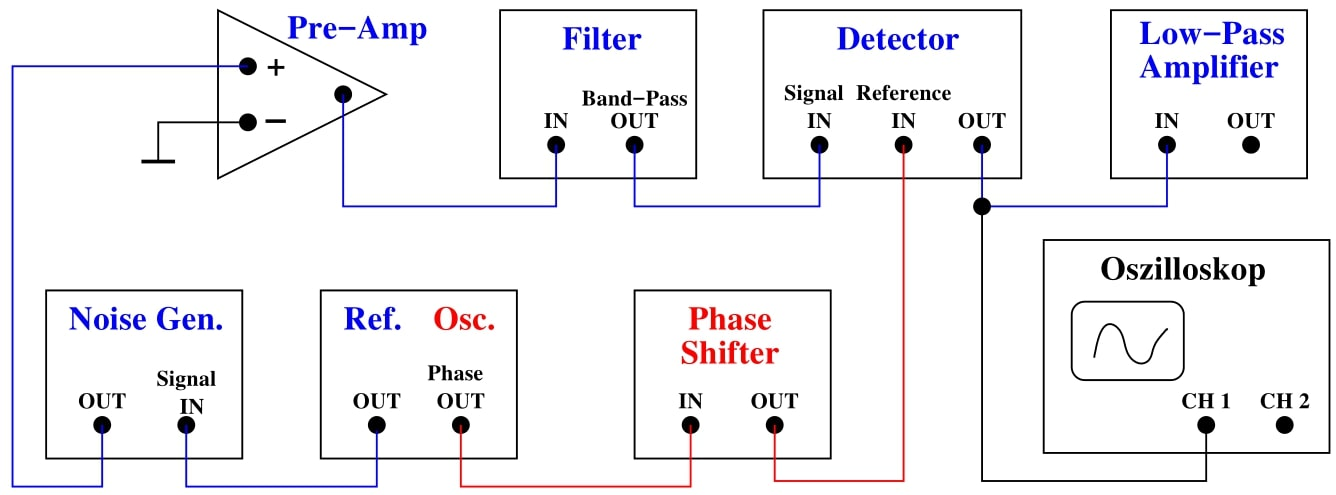
\includegraphics[width=\linewidth]{./images/lock-in.jpg}
    \caption{Versuchsaufbau des Lock-In-Verstärkers \cite{V303}}
    \label{fig:1}
\end{figure}

\flushleft{Zunächst\;}\justifying wird der Noise Generator überbrückt, damit das ungestörte Signal $U_{sig}$ mit dem Referenzsignal $U_{ref}$
im Detektor multipliziert werden kann. Anschließend wird der USB Stick am Oszilloskop angeschlossen und es werden für fünf Phasen das Phasendiagramm 
der multiplizierten Signale gespeichert. Danach soll die Ausgangsspannung in Abhängigkeit der Phase am Tiefpass gemessen werden. Dafür werden 
20 unterschiedliche Phasen am Phase Shifter eingestellt. 

\flushleft{Nun\;}\justifying wird der Noise Generator dazu geschaltet. Für das nun gestörte Signal $U_{sig}$ werden erneut fünf Phasendiagramme
erstellt. Außerdem werden für die selben 20 Phasen wie bei den Messungen ohne Störung die Ausgangsspannung vom Tiefpass abgelesen. 

\flushleft{Anschließend\;}\justifying wird der Aufbau wie in Abbildung \ref{fig:2} abgeändert, sodass nun eine LED und ein Photodetektor den 
Noise Generator ersetzen:

\begin{figure}[H]
    \centering
    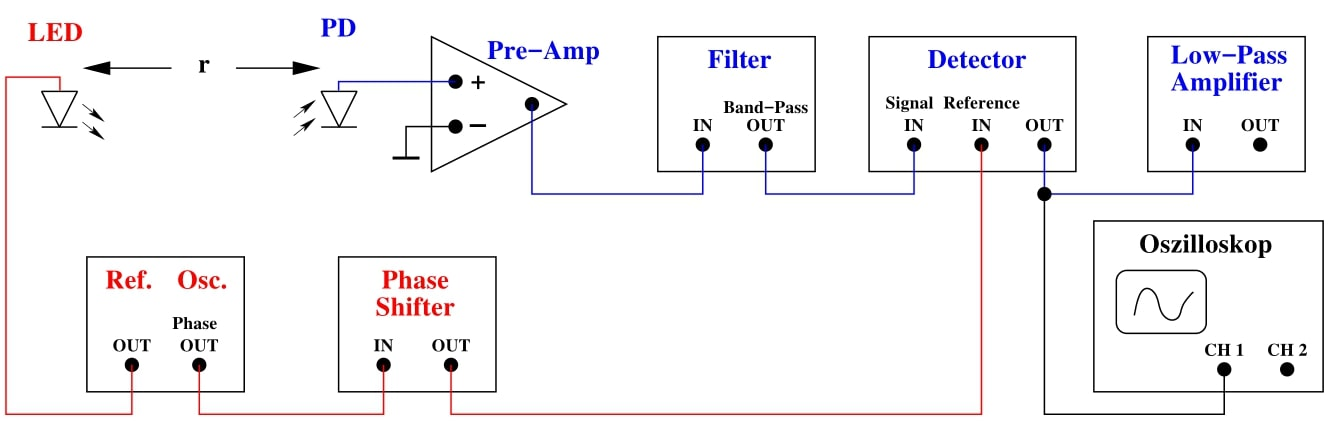
\includegraphics[width=\linewidth]{./images/lock-in_led.jpg}
    \caption{Versuchsaufbau des Lock-In-Verstärkers mit LED \cite{V303}}
    \label{fig:2}
\end{figure}

\flushleft{Die\;}\justifying LED  und der Photodetektor werden auf einer Skala montiert, dabei soll die LED beweglich bleiben und der Detektor stationär.
Die LED wird auf eine Leuchtfrequenz zwischen $\SI{50}{\hertz}$ und $\SI{500}{\hertz}$ eingestellt. Nun wird die LED um gleichmäßige Distanzen
von dem Photodetektor wegbewegt, hier um $\SI{2}{\centi\meter}$. Für jede neue Distanz wird die Intensität am Oszilloskop abgelesen. Sobald sich keine
Änderung der Intensität am Oszilloskop erkennen lässt, werden keine weiteren Messwerte mehr aufgenommen.  

% Auswertung %%%%%%%%%%%%%%%%%%%%%%%%%%%%%%%%%%%%%%%%%%%%%%%%%%%%%%%%%%%%%%%%%%%%%%%%%%%%%%%%%%%%%%%%%%%%%%%%%%%%%%%%%%%%%%%%%%%%%%%%%%%%%%%%%%%%%%%%%%%%%%%%%%%%%%%%%%%%%%%%%%%%%%%%%%%%%%%%%%%%%%%%%%%%%%%%%%

\section{Auswertung} \label{sec:5}

\flushleft{Die\;}\justifying Phasendiagramme der multiplizierten Signale sind in Abbildung \ref{fig:3} dargestellt. Die linke Seite beinhaltet
das multiplizierte Signal ohne Störung und die rechte Seite das mit Störung. Die Phase von $U_{ref}$ wird mit dem Phase Shifter aus Abbildung 
\ref{fig:1} variiert. Die fünf Phasen, mit welchen die Phasendiagramme aufgenommen werden, betragen $\SI{0}{\degree}, \SI{90}{\degree}, 
\SI{135}{\degree}, \SI{180}{\degree}$ und $\SI{270}{\degree}$.

\begin{figure}[H]
\caption{Phasendiagramme}
\label{fig:3}
    \begin{subfigure}{0.495\linewidth} % Phi = 0 --------------------------------------------------------------------------
        \centering
        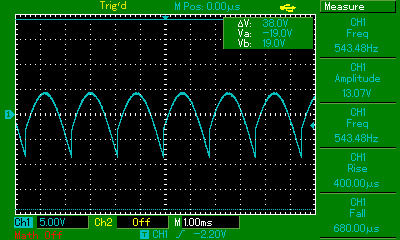
\includegraphics[width=\textwidth]{images/aufg2_phi0.jpg}
        \caption{Phase = $\SI{0}{\degree}$ ohne Störung}
        \label{fig:3a}
    \end{subfigure}
    \begin{subfigure}{0.495\linewidth}
        \centering
        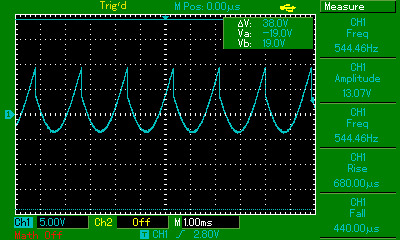
\includegraphics[width=\textwidth]{images/aufg3_phi0.jpg}
        \caption{Phase = $\SI{0}{\degree}$ mit Störung}
        \label{fig:3b}
    \end{subfigure}
    \begin{subfigure}{0.495\linewidth} % Phi = 90 --------------------------------------------------------------------------
        \centering
        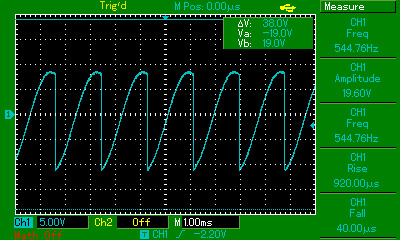
\includegraphics[width=\textwidth]{images/aufg2_phi90.jpg}
        \caption{Phase = $\SI{90}{\degree}$ ohne Störung}
        \label{fig:3c}
    \end{subfigure}
    \begin{subfigure}{0.495\linewidth}
        \centering
        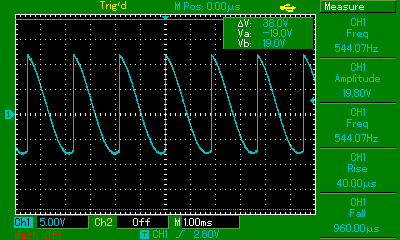
\includegraphics[width=\textwidth]{images/aufg3_phi90.jpg}
        \caption{Phase = $\SI{90}{\degree}$ mit Störung}
        \label{fig:3d}
    \end{subfigure}
    \begin{subfigure}{0.495\linewidth} % Phi = 135 --------------------------------------------------------------------------
        \centering
        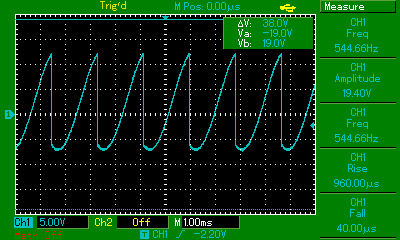
\includegraphics[width=\textwidth]{images/aufg2_phi135.jpg}
        \caption{Phase = $\SI{135}{\degree}$ ohne Störung}
        \label{fig:3e}
    \end{subfigure}
    \begin{subfigure}{0.495\linewidth}
        \centering
        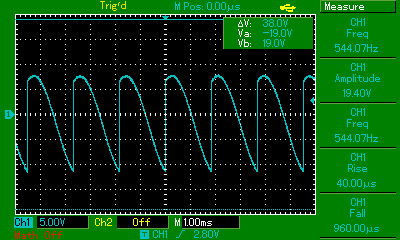
\includegraphics[width=\textwidth]{images/aufg3_phi135.jpg}
        \caption{Phase = $\SI{135}{\degree}$ mit Störung}
        \label{fig:3f}
    \end{subfigure}
    \begin{subfigure}{0.495\linewidth} % Phi = 180 --------------------------------------------------------------------------
        \centering
        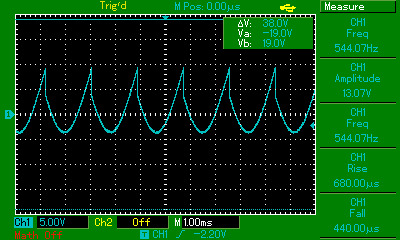
\includegraphics[width=\textwidth]{images/aufg2_phi180.jpg}
        \caption{Phase = $\SI{180}{\degree}$ ohne Störung}
        \label{fig:3g}
    \end{subfigure}
    \begin{subfigure}{0.495\linewidth}
        \centering
        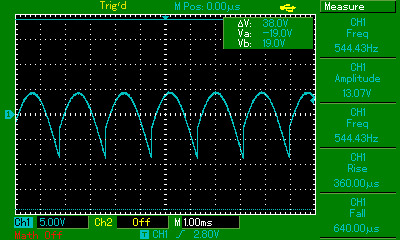
\includegraphics[width=\textwidth]{images/aufg3_phi180.jpg}
        \caption{Phase = $\SI{180}{\degree}$ mit Störung}
        \label{fig:3h}
    \end{subfigure}
    \begin{subfigure}{0.495\linewidth} % Phi = 270 --------------------------------------------------------------------------
        \centering
        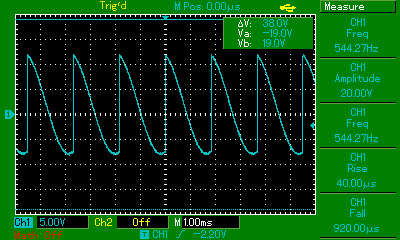
\includegraphics[width=\textwidth]{images/aufg2_phi270.jpg}
        \caption{Phase = $\SI{270}{\degree}$ ohne Störung}
        \label{fig:3i}
    \end{subfigure}
    \begin{subfigure}{0.495\linewidth}
        \centering
        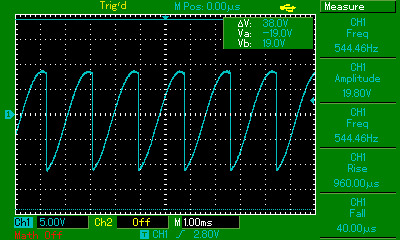
\includegraphics[width=\textwidth]{images/aufg3_phi270.jpg}
        \caption{Phase = $\SI{270}{\degree}$ mit Störung}
        \label{fig:3j}
    \end{subfigure}
\end{figure}

\flushleft{Die\;}\justifying Messwerte für das Integrierte Signal ohne Störung und die dazugehörigen Phasen, sind in der folgenden Tabelle 
\ref{tab:1} aufgetragen:

\begin{table}[H]
    \centering
    \input{table_oS.tex}
    \caption{Messwerte ohne Störung}
    \label{tab:1}
\end{table}

\flushleft{Der\;}\justifying folgenden Graph \ref{fig:4} stellt das Amplitudenverhältnis des integrierten Signals ohne Störung bezüglich der 
Phase dar. Die nicht-lineare Regression wird mit dem Python Befehl np.ployfit() \cite{uncertainties}, der Formel \eqref{eq:1} 
\begin{align}
    U_{out} &= \frac{2}{\pi} \cdot A \cdot \cos(\varphi + B) \label{eq:3}
\intertext{und den folgenden Parametern erstellt:}
    A &= \text{\input{A_os.tex}} \label{eq:4}\\
    B &= \text{\input{B_os.tex}} \label{eq:5}
\end{align}

\begin{figure}[H]
    \centering
    \includegraphics[width=0.75\linewidth]{plotphi_oS.pdf}
    \caption{Nicht-lineare Regression des Signals ohne Störung}
    \label{fig:4}
\end{figure}

\flushleft{Die\;}\justifying Messwerte des integrierten Signals mit Störung und die dazugehörigen Phasen sind in der folgenden Tabelle
\ref{tab:2} aufgelistet:

\begin{table}[H]
    \centering
    \input{table_mS.tex}
    \caption{Messwerte mit Störung}
    \label{tab:2}
\end{table}

\flushleft{Der\;}\justifying folgende Graph \ref{fig:4} stellt das Amplitudenverhältnis des integrierten Signals mit Störung bezüglich der 
Phase dar. Dieser Graph wird ebenso mit dem Python Befehl np.ployfit() \cite{uncertainties}, der Formel \eqref{eq:1} 
\begin{align}
    U_{out} &= \frac{2}{\pi} \cdot C \cdot \cos(\varphi + D) \label{eq:6}
\intertext{und den folgenden Parametern erstellt:}
    C &= \text{\input{A_ms.tex}} \label{eq:7}\\
    D &= \text{\input{B_ms.tex}} \label{eq:8}
\end{align}

\begin{figure}[H]
    \centering
    \includegraphics[width=0.75\linewidth]{plotphi_mS.pdf}
    \caption{Nicht-lineare Regression des Signals mit Störung}
    \label{fig:5}
\end{figure}

\flushleft{Die\;}\justifying folgende Tabelle gibt die Messwerte der Intensität der LED aus Abbildung \ref{fig:2} bezüglich des gemessenen 
Abstands wieder:

\begin{table}[H]
    \centering
    \input{table_I.tex}
    \caption{Messwerte der Intensität}
    \label{tab:3}
\end{table}

\flushleft{Die\;}\justifying Kurve der Intensität mit der Funktion
\begin{subequations}
\begin{align}
    I&=E \frac{1}{r^2}+F 
    \intertext{und den Fitparametern}
    E&=\text{\input{I_A.tex} \quad \text{und}}\\
    F&=\text{\input{I_B.tex}}
\end{align}
\end{subequations}
\flushleft{sieht\;}\justifying aus wie folgt:

\begin{figure}[H]
    \centering
    \includegraphics[width=0.75\linewidth]{plotI.pdf}
    \caption{Nicht-lineare Regression der Intensität}
    \label{fig:6}
\end{figure}

% Diskussion %%%%%%%%%%%%%%%%%%%%%%%%%%%%%%%%%%%%%%%%%%%%%%%%%%%%%%%%%%%%%%%%%%%%%%%%%%%%%%%%%%%%%%%%%%%%%%%%%%%%%%%%%%%%%%%%%%%%%%%%%%%%%%%%%%%%%%%%%%%%%%%%%%%%%%%%%%%%%%%%%%%%%%%%%%%%%%%%%%%%%%%%%%%%%%%%%%

\section{Diskussion} \label{sec:6}

\flushleft{Es\;}\justifying lässt sich in Abbildung \ref{fig:3} erkennen, dass sich das ungestörte Signal und das gestörte Signal ähneln. Unter 
genauerer Betrachtung lässt sich feststellen, dass der Unterschied zwischen den Graphen in der Phasenverschiebung von ungefähr $\sfrac{\pi}{2}$
liegt. Abgesehen von den leicht unterschiedlichen Phasenverläufen, sind die Amplituden identisch. 


\flushleft{Die\;}\justifying folgenden Abbildungen zeigen die Parameter der Signale $U_{ref}$ (CH1) und $U_{sig}$ (CH2). Hier ist $U_{ref}$ (CH1)
das variable Signal.

\begin{figure}[H] 
\caption{Funktionalität des Gleichrichters}
\label{fig:7}
    \begin{subfigure}{0.495\linewidth}
        \centering
        \includegraphics[width=\textwidth]{images/ungestört_graph.jpg}
        \caption{Phasendiagramm der Signale $U_{sig}$ und $U_{ref}$}
        \label{fig:7a}
    \end{subfigure}
    \begin{subfigure}{0.495\linewidth}
        \centering
        \includegraphics[width=\textwidth]{images/Aconst_ungestört_param.jpg}
        \caption{Parameter des Signals $U_{sig}$}
        \label{fig:7b}
    \end{subfigure}
\end{figure}

\flushleft{Da\;}\justifying das angelegte Signal $U_{sig}$ das zu störende Signal ist, wird der Verstärkungsfakor relevant.
Anhand des Graphen \ref{fig:4} ohne Störung und dessen Parameter $A$ \eqref{eq:4}, welcher laut Formel \eqref{eq:1} die angelegte Spannung $U_0$ 
beschreibt, lässt sich $U_0$ bestimmen als:
\begin{align}
    U_0 = A = \text{\input{A_os.tex}}
\end{align}
Wird diese Spannung mit der Amplitude $U = \SI{6.57}{\volt}$ aus Abbildung \ref{fig:7b}, welche von Reference/Oscillator ausgegeben wird, verglichen, 
lässt sich ein Verstärkungsfakor von $\sfrac{U_0}{U} = \text{\input{faktor_os.tex}}$ berechnen. Der Graph \ref{fig:4} gibt einen erwarteten Amplitudenverlauf 
des Signals $U_{sig}$ ohne Störung wieder. 

\flushleft{Aus\;}\justifying dem Graphen \ref{fig:5} des Signals mit Störung und dessen Parameter $C$ lässt sich die angelegte Spannung 
\begin{align}
    U_0 = C = \text{\input{A_ms.tex}}
\end{align}
analog zum Graphen ohne Störung bestimmen. Um den Verstärkungsfakor zu berechnen, wird hier ebenfalls die Amplitude $U = \SI{6.57}{\volt}$ aus 
Abbildung \ref{fig:7b} verwendet. Daraus folgt der Verstärkungsfakor des Signals von $\sfrac{U_0}{U} = \text{\input{faktor_ms.tex}}$ mit Störung.

\flushleft{Der\;}\justifying Graph \ref{fig:6} gibt die abklingende Genauigkeit des empfangenen Signals der LED wieder. Die Intensität aus Tabelle
\ref{tab:3} sollte mit einem Faktor von $\sfrac{1}{r^2}$ abfallen. Dies ist hier jedoch nicht der Fall. Die nicht-lineare Regression aus \ref{fig:6} 
zeigt das eigentliche Verhalten der Intensität. Die Messwerte verhalten sich jedoch anders. Dies könnte mit dem wackeligen Aufbau des Photodetektors
zusammenhängen, oder einer hohen Intensität der Hintergrundstrahlung.
% Literatur %%%%%%%%%%%%%%%%%%%%%%%%%%%%%%%%%%%%%%%%%%%%%%%%%%%%%%%%%%%%%%%%%%%%%%%%%%%%%%%%%%%%%%%%%%%%%%%%%%%%%%%%%%%%%%%%%%%%%%%%%%%%%%%%%%%%%%%%%%%%%%%%%%%%%%%%%%%%%%%%%%%%%%%%%%%%%%%%%%%%%%%%%%%%%%%%%%

\newpage
\printbibliography

\end{document}